
\documentclass[10pt,journal,compsoc]{IEEEtran}
% *** CITATION PACKAGES ***
%
\ifCLASSOPTIONcompsoc
  % IEEE Computer Society needs nocompress option
  % requires cite.sty v4.0 or later (November 2003)
  \usepackage[nocompress]{cite}
\else
  % normal IEEE
  \usepackage{cite}
\fi

\usepackage{subfigure}
\usepackage{hyperref}
\usepackage{url}
\usepackage{pifont}
\usepackage[usenames]{color,colortbl}
 \setlength\arraycolsep{1pt}
 \definecolor{MyLightCyan}{rgb}{0,1.0,1.0}

\usepackage{graphicx}
\graphicspath{{image/}{pdf/}{fig/}{svg/}}
\DeclareGraphicsExtensions{.fig,.pdf,.png,.jpg}
\usepackage{figlatex}
\begin{document}
\title{Through The Coherency Port: The Adventures of a FPGA Trojan}
\author{Sumanta~Chaudhuri}
\IEEEtitleabstractindextext{%
\begin{abstract}
The abstract goes here.
\end{abstract}

% Note that keywords are not normally used for peerreview papers.
\begin{IEEEkeywords}
Computer Society, IEEE, IEEEtran, journal, \LaTeX, paper, template.
\end{IEEEkeywords}}


% make the title area
\maketitle


\section{Introduction}

\begin{figure*}[!t]
\centering
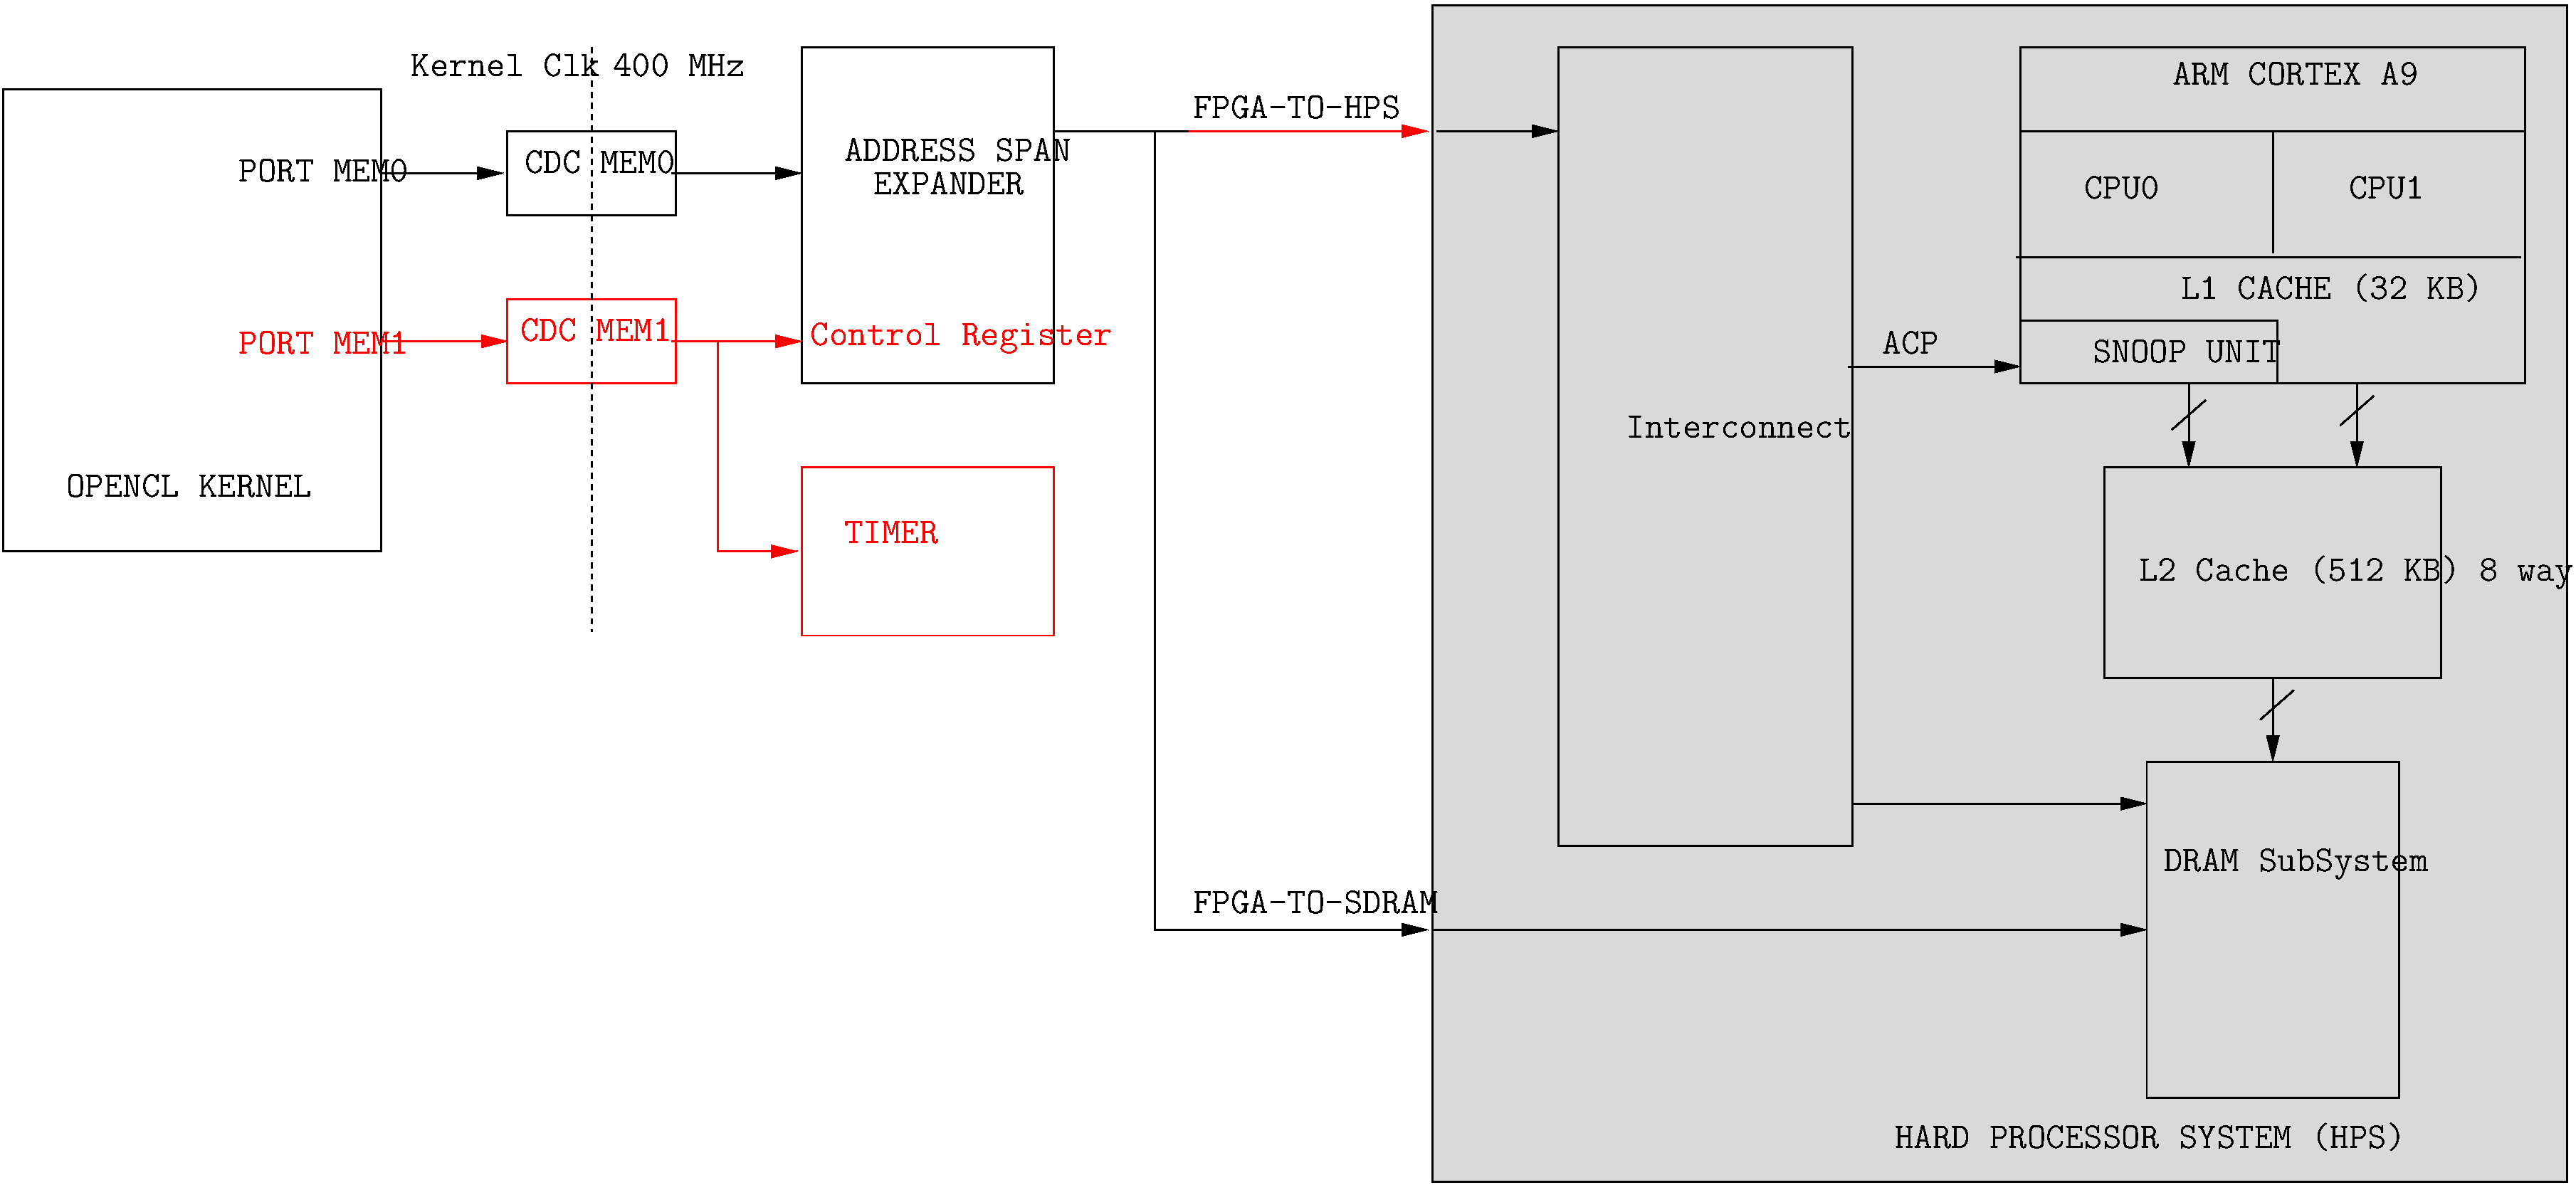
\includegraphics[width=0.8\textwidth]{./fig/opencl.pdf}
\caption{Customised Opencl Platform for the FPGA Trojan}
\label{fig_dlcs}
\end{figure*}



\end{document}
